\begin{minipage}{0.63\textwidth}
    \parskip=1em
    \section*{セキュリティモジュール:3つのダイヤル}
    
    \uline{概要}:A, B, Cと表示されている3つのダイヤルと一文字のディスプレイ、そしてOKボタンがあります。

    \uline{解除方法}:3つのダイヤルを正しい数字を指すように回してOKボタンを押してください。
\end{minipage}%
\hfill%
\begin{minipage}{0.33\textwidth}
    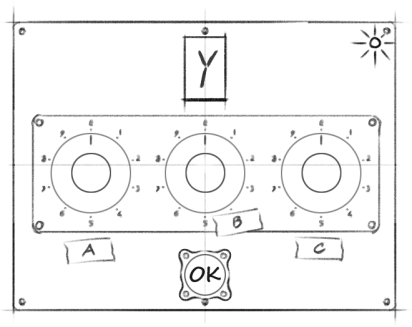
\includegraphics[width=\textwidth]{images/64.png}
    \vspace*{\fill}
\end{minipage}

\uline{ダイヤルA}:ダイヤルを回して、音が再生される値と、文字ディスプレイに「{X}」が表示される値を観察します。

\bgroup
\fontsize{9.5}{9.5}\selectfont
\begin{tabular}{|p{0.3\textwidth}p{0.3\textwidth}p{0.3\textwidth}|}
    \hline
    \multicolumn{3}{|c|}{ダイヤルA}\\ \hline
    \multicolumn{1}{|>{\centering}p{0.3\textwidth}|}{音が鳴る値} &
    \multicolumn{1}{|>{\centering}p{0.3\textwidth}|}{「{X}」が表示される値} &
    \multicolumn{1}{|>{\centering}p{0.3\textwidth}|}{正しいダイヤルAの値} \\ \hline
    \multicolumn{1}{|>{\centering}p{0.3\textwidth}|}{2} &
    \multicolumn{1}{|>{\centering}p{0.3\textwidth}|}{5} &
    \multicolumn{1}{|>{\centering}p{0.3\textwidth}|}{1} \\ \hline
    \multicolumn{1}{|>{\centering}p{0.3\textwidth}|}{2} &
    \multicolumn{1}{|>{\centering}p{0.3\textwidth}|}{3} &
    \multicolumn{1}{|>{\centering}p{0.3\textwidth}|}{2} \\ \hline
    \multicolumn{1}{|>{\centering}p{0.3\textwidth}|}{2} &
    \multicolumn{1}{|>{\centering}p{0.3\textwidth}|}{6} &
    \multicolumn{1}{|>{\centering}p{0.3\textwidth}|}{3} \\ \hline
    %
    \multicolumn{1}{|>{\centering}p{0.3\textwidth}|}{4} &
    \multicolumn{1}{|>{\centering}p{0.3\textwidth}|}{8} &
    \multicolumn{1}{|>{\centering}p{0.3\textwidth}|}{4} \\ \hline
    \multicolumn{1}{|>{\centering}p{0.3\textwidth}|}{4} &
    \multicolumn{1}{|>{\centering}p{0.3\textwidth}|}{7} &
    \multicolumn{1}{|>{\centering}p{0.3\textwidth}|}{5} \\ \hline
    %
    \multicolumn{1}{|>{\centering}p{0.3\textwidth}|}{6} &
    \multicolumn{1}{|>{\centering}p{0.3\textwidth}|}{0} &
    \multicolumn{1}{|>{\centering}p{0.3\textwidth}|}{6} \\ \hline
    \multicolumn{1}{|>{\centering}p{0.3\textwidth}|}{6} &
    \multicolumn{1}{|>{\centering}p{0.3\textwidth}|}{1} &
    \multicolumn{1}{|>{\centering}p{0.3\textwidth}|}{7} \\ \hline
    %
    \multicolumn{1}{|>{\centering}p{0.3\textwidth}|}{7} &
    \multicolumn{1}{|>{\centering}p{0.3\textwidth}|}{3} &
    \multicolumn{1}{|>{\centering}p{0.3\textwidth}|}{8} \\ \hline
    \multicolumn{1}{|>{\centering}p{0.3\textwidth}|}{7} &
    \multicolumn{1}{|>{\centering}p{0.3\textwidth}|}{6} &
    \multicolumn{1}{|>{\centering}p{0.3\textwidth}|}{9} \\ \hline
    \multicolumn{1}{|>{\centering}p{0.3\textwidth}|}{7} &
    \multicolumn{1}{|>{\centering}p{0.3\textwidth}|}{1} &
    \multicolumn{1}{|>{\centering}p{0.3\textwidth}|}{0} \\ \hline
    %
    \multicolumn{1}{|>{\centering}p{0.3\textwidth}|}{1} &
    \multicolumn{1}{|>{\centering}p{0.3\textwidth}|}{3} &
    \multicolumn{1}{|>{\centering}p{0.3\textwidth}|}{1} \\ \hline
    \multicolumn{1}{|>{\centering}p{0.3\textwidth}|}{1} &
    \multicolumn{1}{|>{\centering}p{0.3\textwidth}|}{7} &
    \multicolumn{1}{|>{\centering}p{0.3\textwidth}|}{2} \\ \hline
    \multicolumn{1}{|>{\centering}p{0.3\textwidth}|}{1} &
    \multicolumn{1}{|>{\centering}p{0.3\textwidth}|}{9} &
    \multicolumn{1}{|>{\centering}p{0.3\textwidth}|}{3} \\ \hline
    %
    \multicolumn{1}{|>{\centering}p{0.3\textwidth}|}{3} &
    \multicolumn{1}{|>{\centering}p{0.3\textwidth}|}{1} &
    \multicolumn{1}{|>{\centering}p{0.3\textwidth}|}{4} \\ \hline
    \multicolumn{1}{|>{\centering}p{0.3\textwidth}|}{3} &
    \multicolumn{1}{|>{\centering}p{0.3\textwidth}|}{5} &
    \multicolumn{1}{|>{\centering}p{0.3\textwidth}|}{5} \\ \hline
    %
    \multicolumn{1}{|>{\centering}p{0.3\textwidth}|}{5} &
    \multicolumn{1}{|>{\centering}p{0.3\textwidth}|}{8} &
    \multicolumn{1}{|>{\centering}p{0.3\textwidth}|}{6} \\ \hline
    \multicolumn{1}{|>{\centering}p{0.3\textwidth}|}{5} &
    \multicolumn{1}{|>{\centering}p{0.3\textwidth}|}{2} &
    \multicolumn{1}{|>{\centering}p{0.3\textwidth}|}{7} \\ \hline
    %
    \multicolumn{1}{|>{\centering}p{0.3\textwidth}|}{8} &
    \multicolumn{1}{|>{\centering}p{0.3\textwidth}|}{4} &
    \multicolumn{1}{|>{\centering}p{0.3\textwidth}|}{8} \\ \hline
    \multicolumn{1}{|>{\centering}p{0.3\textwidth}|}{8} &
    \multicolumn{1}{|>{\centering}p{0.3\textwidth}|}{0} &
    \multicolumn{1}{|>{\centering}p{0.3\textwidth}|}{9} \\ \hline
    %
    \multicolumn{1}{|>{\centering}p{0.3\textwidth}|}{9} &
    \multicolumn{1}{|>{\centering}p{0.3\textwidth}|}{7} &
    \multicolumn{1}{|>{\centering}p{0.3\textwidth}|}{0} \\ \hline
\end{tabular}
\egroup

\uline{ダイヤルB}:ダイヤルを回して、文字ディスプレイに「{X}」と「{Z}」が表示される値を観察します。

\bgroup
\fontsize{9.5}{9.5}\selectfont
\begin{tabular}{|p{0.3\textwidth}p{0.3\textwidth}p{0.3\textwidth}|}
    \hline
    \multicolumn{3}{|c|}{ダイヤルB}\\ \hline
    \multicolumn{1}{|>{\centering}p{0.3\textwidth}|}{「{X}」が表示される値} &
    \multicolumn{1}{|>{\centering}p{0.3\textwidth}|}{「{Z}」が表示される値} &
    \multicolumn{1}{|>{\centering}p{0.3\textwidth}|}{正しいダイヤルBの値} \\ \hline
    \multicolumn{1}{|>{\centering}p{0.3\textwidth}|}{0} &
    \multicolumn{1}{|>{\centering}p{0.3\textwidth}|}{9} &
    \multicolumn{1}{|>{\centering}p{0.3\textwidth}|}{7} \\ \hline
    \multicolumn{1}{|>{\centering}p{0.3\textwidth}|}{0} &
    \multicolumn{1}{|>{\centering}p{0.3\textwidth}|}{8} &
    \multicolumn{1}{|>{\centering}p{0.3\textwidth}|}{1} \\ \hline
    \multicolumn{1}{|>{\centering}p{0.3\textwidth}|}{0} &
    \multicolumn{1}{|>{\centering}p{0.3\textwidth}|}{4} &
    \multicolumn{1}{|>{\centering}p{0.3\textwidth}|}{9} \\ \hline
    %
    \multicolumn{1}{|>{\centering}p{0.3\textwidth}|}{1} &
    \multicolumn{1}{|>{\centering}p{0.3\textwidth}|}{3} &
    \multicolumn{1}{|>{\centering}p{0.3\textwidth}|}{0} \\ \hline
    \multicolumn{1}{|>{\centering}p{0.3\textwidth}|}{1} &
    \multicolumn{1}{|>{\centering}p{0.3\textwidth}|}{2} &
    \multicolumn{1}{|>{\centering}p{0.3\textwidth}|}{0} \\ \hline
    \multicolumn{1}{|>{\centering}p{0.3\textwidth}|}{1} &
    \multicolumn{1}{|>{\centering}p{0.3\textwidth}|}{6} &
    \multicolumn{1}{|>{\centering}p{0.3\textwidth}|}{8} \\ \hline
    %
    \multicolumn{1}{|>{\centering}p{0.3\textwidth}|}{2} &
    \multicolumn{1}{|>{\centering}p{0.3\textwidth}|}{1} &
    \multicolumn{1}{|>{\centering}p{0.3\textwidth}|}{5} \\ \hline
    \multicolumn{1}{|>{\centering}p{0.3\textwidth}|}{2} &
    \multicolumn{1}{|>{\centering}p{0.3\textwidth}|}{3} &
    \multicolumn{1}{|>{\centering}p{0.3\textwidth}|}{3} \\ \hline
    \multicolumn{1}{|>{\centering}p{0.3\textwidth}|}{2} &
    \multicolumn{1}{|>{\centering}p{0.3\textwidth}|}{8} &
    \multicolumn{1}{|>{\centering}p{0.3\textwidth}|}{8} \\ \hline
    %
    \multicolumn{1}{|>{\centering}p{0.3\textwidth}|}{3} &
    \multicolumn{1}{|>{\centering}p{0.3\textwidth}|}{5} &
    \multicolumn{1}{|>{\centering}p{0.3\textwidth}|}{1} \\ \hline
    \multicolumn{1}{|>{\centering}p{0.3\textwidth}|}{3} &
    \multicolumn{1}{|>{\centering}p{0.3\textwidth}|}{4} &
    \multicolumn{1}{|>{\centering}p{0.3\textwidth}|}{6} \\ \hline
    \multicolumn{1}{|>{\centering}p{0.3\textwidth}|}{3} &
    \multicolumn{1}{|>{\centering}p{0.3\textwidth}|}{0} &
    \multicolumn{1}{|>{\centering}p{0.3\textwidth}|}{1} \\ \hline
    %
    \multicolumn{1}{|>{\centering}p{0.3\textwidth}|}{4} &
    \multicolumn{1}{|>{\centering}p{0.3\textwidth}|}{3} &
    \multicolumn{1}{|>{\centering}p{0.3\textwidth}|}{5} \\ \hline
    \multicolumn{1}{|>{\centering}p{0.3\textwidth}|}{4} &
    \multicolumn{1}{|>{\centering}p{0.3\textwidth}|}{2} &
    \multicolumn{1}{|>{\centering}p{0.3\textwidth}|}{5} \\ \hline
    \multicolumn{1}{|>{\centering}p{0.3\textwidth}|}{4} &
    \multicolumn{1}{|>{\centering}p{0.3\textwidth}|}{5} &
    \multicolumn{1}{|>{\centering}p{0.3\textwidth}|}{1} \\ \hline
    %
\end{tabular}
\egroup

\bgroup
\fontsize{9.5}{9.5}\selectfont
\begin{tabular}{|p{0.3\textwidth}p{0.3\textwidth}p{0.3\textwidth}|}
    \hline
    \multicolumn{3}{|c|}{ダイヤルB}\\ \hline
    \multicolumn{1}{|>{\centering}p{0.3\textwidth}|}{「{X}」が表示される値} &
    \multicolumn{1}{|>{\centering}p{0.3\textwidth}|}{「{Z}」が表示される値} &
    \multicolumn{1}{|>{\centering}p{0.3\textwidth}|}{正しいダイヤルBの値} \\ \hline
    %
    \multicolumn{1}{|>{\centering}p{0.3\textwidth}|}{5} &
    \multicolumn{1}{|>{\centering}p{0.3\textwidth}|}{7} &
    \multicolumn{1}{|>{\centering}p{0.3\textwidth}|}{1} \\ \hline
    \multicolumn{1}{|>{\centering}p{0.3\textwidth}|}{5} &
    \multicolumn{1}{|>{\centering}p{0.3\textwidth}|}{6} &
    \multicolumn{1}{|>{\centering}p{0.3\textwidth}|}{4} \\ \hline
    \multicolumn{1}{|>{\centering}p{0.3\textwidth}|}{5} &
    \multicolumn{1}{|>{\centering}p{0.3\textwidth}|}{9} &
    \multicolumn{1}{|>{\centering}p{0.3\textwidth}|}{1} \\ \hline
    %
    \multicolumn{1}{|>{\centering}p{0.3\textwidth}|}{6} &
    \multicolumn{1}{|>{\centering}p{0.3\textwidth}|}{5} &
    \multicolumn{1}{|>{\centering}p{0.3\textwidth}|}{4} \\ \hline
    \multicolumn{1}{|>{\centering}p{0.3\textwidth}|}{6} &
    \multicolumn{1}{|>{\centering}p{0.3\textwidth}|}{8} &
    \multicolumn{1}{|>{\centering}p{0.3\textwidth}|}{1} \\ \hline
    \multicolumn{1}{|>{\centering}p{0.3\textwidth}|}{6} &
    \multicolumn{1}{|>{\centering}p{0.3\textwidth}|}{1} &
    \multicolumn{1}{|>{\centering}p{0.3\textwidth}|}{4} \\ \hline
    %
    \multicolumn{1}{|>{\centering}p{0.3\textwidth}|}{7} &
    \multicolumn{1}{|>{\centering}p{0.3\textwidth}|}{1} &
    \multicolumn{1}{|>{\centering}p{0.3\textwidth}|}{8} \\ \hline
    \multicolumn{1}{|>{\centering}p{0.3\textwidth}|}{7} &
    \multicolumn{1}{|>{\centering}p{0.3\textwidth}|}{4} &
    \multicolumn{1}{|>{\centering}p{0.3\textwidth}|}{1} \\ \hline
    \multicolumn{1}{|>{\centering}p{0.3\textwidth}|}{7} &
    \multicolumn{1}{|>{\centering}p{0.3\textwidth}|}{3} &
    \multicolumn{1}{|>{\centering}p{0.3\textwidth}|}{0} \\ \hline
    %
    \multicolumn{1}{|>{\centering}p{0.3\textwidth}|}{8} &
    \multicolumn{1}{|>{\centering}p{0.3\textwidth}|}{4} &
    \multicolumn{1}{|>{\centering}p{0.3\textwidth}|}{6} \\ \hline
    \multicolumn{1}{|>{\centering}p{0.3\textwidth}|}{8} &
    \multicolumn{1}{|>{\centering}p{0.3\textwidth}|}{2} &
    \multicolumn{1}{|>{\centering}p{0.3\textwidth}|}{8} \\ \hline
    \multicolumn{1}{|>{\centering}p{0.3\textwidth}|}{8} &
    \multicolumn{1}{|>{\centering}p{0.3\textwidth}|}{7} &
    \multicolumn{1}{|>{\centering}p{0.3\textwidth}|}{9} \\ \hline
    %
    \multicolumn{1}{|>{\centering}p{0.3\textwidth}|}{9} &
    \multicolumn{1}{|>{\centering}p{0.3\textwidth}|}{0} &
    \multicolumn{1}{|>{\centering}p{0.3\textwidth}|}{5} \\ \hline
    \multicolumn{1}{|>{\centering}p{0.3\textwidth}|}{9} &
    \multicolumn{1}{|>{\centering}p{0.3\textwidth}|}{7} &
    \multicolumn{1}{|>{\centering}p{0.3\textwidth}|}{5} \\ \hline
    \multicolumn{1}{|>{\centering}p{0.3\textwidth}|}{9} &
    \multicolumn{1}{|>{\centering}p{0.3\textwidth}|}{5} &
    \multicolumn{1}{|>{\centering}p{0.3\textwidth}|}{3} \\ \hline
    %
\end{tabular}
\egroup

\uline{ダイヤルC}:ダイヤルAとBを正しい方向にして、タイマーの最後の2桁を確認します。

\bgroup
\fontsize{9.5}{9.5}\selectfont
\begin{tabular}{|p{0.3\textwidth}p{0.3\textwidth}p{0.3\textwidth}|}
    \hline
    \multicolumn{3}{|c|}{ダイヤルC}\\ \hline
    \multicolumn{1}{|>{\centering}p{0.3\textwidth}|}{ダイヤルAとBの値の合計が} &
    \multicolumn{1}{|>{\centering}p{0.3\textwidth}|}{タイマーの最後の2桁} &
    \multicolumn{1}{|>{\centering}p{0.3\textwidth}|}{正しいダイヤルCの値} \\ \hline
    \multicolumn{1}{|>{\centering}p{0.3\textwidth}|}{偶数} &
    \multicolumn{1}{|>{\centering}p{0.3\textwidth}|}{0-15秒} &
    \multicolumn{1}{|>{\centering}p{0.3\textwidth}|}{1} \\ \hline
    \multicolumn{1}{|>{\centering}p{0.3\textwidth}|}{偶数} &
    \multicolumn{1}{|>{\centering}p{0.3\textwidth}|}{16-30秒} &
    \multicolumn{1}{|>{\centering}p{0.3\textwidth}|}{2} \\ \hline
    \multicolumn{1}{|>{\centering}p{0.3\textwidth}|}{偶数} &
    \multicolumn{1}{|>{\centering}p{0.3\textwidth}|}{31-45秒} &
    \multicolumn{1}{|>{\centering}p{0.3\textwidth}|}{3} \\ \hline
    \multicolumn{1}{|>{\centering}p{0.3\textwidth}|}{偶数} &
    \multicolumn{1}{|>{\centering}p{0.3\textwidth}|}{46-59秒} &
    \multicolumn{1}{|>{\centering}p{0.3\textwidth}|}{4} \\ \hline
    \multicolumn{1}{|>{\centering}p{0.3\textwidth}|}{奇数} &
    \multicolumn{1}{|>{\centering}p{0.3\textwidth}|}{0-15秒} &
    \multicolumn{1}{|>{\centering}p{0.3\textwidth}|}{1} \\ \hline
    \multicolumn{1}{|>{\centering}p{0.3\textwidth}|}{奇数} &
    \multicolumn{1}{|>{\centering}p{0.3\textwidth}|}{16-30秒} &
    \multicolumn{1}{|>{\centering}p{0.3\textwidth}|}{2} \\ \hline
    \multicolumn{1}{|>{\centering}p{0.3\textwidth}|}{奇数} &
    \multicolumn{1}{|>{\centering}p{0.3\textwidth}|}{31-45秒} &
    \multicolumn{1}{|>{\centering}p{0.3\textwidth}|}{3} \\ \hline
    \multicolumn{1}{|>{\centering}p{0.3\textwidth}|}{奇数} &
    \multicolumn{1}{|>{\centering}p{0.3\textwidth}|}{46-59秒} &
    \multicolumn{1}{|>{\centering}p{0.3\textwidth}|}{4} \\ \hline
    %
\end{tabular}
\egroup

「まだ生きている爆発物処理班」の為のヒント:
\begin{itemize}
    \item[$\bullet$] ダイヤルAとBを設定する時はゆっくりしても大丈夫です。 ただし、ダイヤルCを設定する時はできるだけ早く実行し、「{OK}」を押してください。
    \item[$\bullet$] 正しい組み合わせを設定しましたが、モジュールはまだ解除されてませんか?ダイヤルが正しい値に正確に設定されていることを確認してください。
\end{itemize}

